
%\documentclass[12pt,twocolumn]{article}
\documentclass[12pt]{article}
\usepackage[spanish,english]{babel}
%\usepackage[spanish]{babel}
\usepackage[utf8]{inputenc}
\usepackage{graphicx}
\usepackage{epsfig}
\usepackage{multicol,caption}
\usepackage{amsthm} % Theorem Formatting
\usepackage{amssymb}    % Math symbols such as \mathbb
\usepackage{color}

\usepackage{hyperref}
\usepackage[none]{hyphenat} 

%\renewcommand{\tablename}{Tabla}
%\def\tablename{Cuadro}% por \def\tablename{Tabla}% 
\newenvironment{Figure}
{\par\medskip\noindent\minipage{\linewidth}}
{\endminipage\par\medskip}

\addto\captionsspanish{%
  \def\tablename{Tabla}%
}

\topmargin  = 10pt
\oddsidemargin  = -0.5in
%\headheight = 12pt
%\headsep    = 15pt
%\footskip   = 15pt
\textheight = 21.5 cm
\textwidth  = 18.5cm

\tolerance=10000

\title{\bf{Experimento demostrativo del periodo de oscilación del péndulo simple, para el aula de clase}}
\author{Julian Salamanca\footnote{jasalamanca@udistrital.edu.co}, Diego Parra\footnote{diegoestudianteud1@gmail.com} \\
  Universidad Distrital, Calle 3 No 26A-40 Bogotá-Colombia\\
  Grupo Física e Informática ``FISINFOR''
}
\date{\today}
\begin{document}
%\def\tablename{Cuadro}% por \def\tablename{Tabla}% 
\renewcommand{\tablename}{Tabla}
\maketitle
\vspace{-0.8cm}

\begin{abstract}
This article provides an educational tool for displaying the oscillation period of the simple pendulum and harmonic movement, an experimental arrangement of an infrared sensor type both sender and receiver, which is operated by a atmega microcontroller 328P-Pu illustrated, sends data through a module HC-06 Bluetooth to a computer with an operating system GNU-Linux family as it is Linux Mint 17 Xfce, which analyzes real-time graphical and we provides important data on the characterization of the system rope – mass, in a controlled infrared radiation and vibrations that can alter our system pendulum swing environment; besides demonstration, the whole project was done with free software and hardware, is an experience that generates classroom projects `` doing physical ''.\\

{\bf{Keywords:}} Pendulum and simple harmonic motion, physics education, free software and hardware..
\end{abstract}
\selectlanguage{spanish}
\begin{abstract}

El presente artículo aporta una herramienta didáctica para la visualización del periodo de oscilación del péndulo  simple y el movimiento armónico,  se ilustra una disposición experimental de un sensor de tipo infrarrojo  tanto emisor como receptor,  el cual es operado por un microcontrolador atmega 328P-Pu, envía datos a través  un modulo bluetooth hc-06 a un ordenador con un sistema operativo de la familia GNU-Linux como lo es Linux Mint 17 xfce, el cual los analiza, gráfica en tiempo real  y nos arroja  datos importantes sobre la caracterización del sistema cuerda – masa, en un ambiente controlado de radiación infrarroja y vibraciones que puedan alterar nuestro sistema de  oscilación del péndulo; además de demostrativo, todo el proyecto fue realizado con software y hardware libre, es una experiencia que permite generar proyectos de aula ``haciendo física''.\\

{\bf{Descriptores:}} Péndulo y movimiento armónico simple, enseñanza de la física, software y hardware libre.
\end{abstract}

\begin{multicols}{2}

\section{Introducción}
Los experimentos demostrativos son utilizados en sesiones magistrales de clase para visualizar y obtener una imagen de la experiencia física, cuyo objetivo primordial es, el hacer participación interactiva con el estudiante\cite{REDISH} en el estudio de los conceptos físicos involucrados. Sin embargo, hay una gran cantidad de conceptos en física que pueden ser ilustrados a través de una simulación o de un arreglo experimental sofisticado.\\ \\ Este artículo presenta una propuesta de experimento para el estudio del periodo de oscilación en un péndulo, el cual busca ser, además de demostrativo, una experiencia que permita generar proyectos de aula ``haciendo física''.
\\ \\

\section{Configuración experimental}
El primer hombre dedicado a la investigación\cite{GALILEO} y realizador de grandes descubrimientos entre ellos la explicación física del péndulo y considerado el primer observador de la ciencia fue el señor Galileo Galilei, el cual dijo acerca de este tópico que sin importar cuál es el espacio de oscilación de un péndulo, siempre tendrá el mismo ritmo. 
\\ \\
El arreglo experimental esta esquematizado en la Fig. 1 y constaba de una cuerda atada a un apoyo, una masa sujeta a la cuerda, y como en aquel tiempo los relojes eran muy escasos, el señor Galilei\cite{GALILEO} utilizo los pulsos que generaba los latidos de su corazón para medir el tiempo.
\\\\
\begin{Figure}
\center
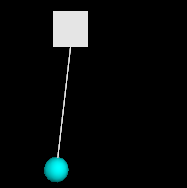
\includegraphics[width=4.0cm, height=5cm] {fig/fig1.png}
\captionof{figure}{Esquema ``Figura realizada en python-visual'' de la configuración experimental utilizada por el señor Galileo Galilei para medir el periodo de oscilación de un péndulo y su isocronismo.}
\label{fig:g1}
\end{Figure}

\subsection{Elaboración del instrumento de medición}

\subsubsection{Materiales}
Para la realización de este montaje se debe utilizar los siguientes componentes:
\begin{enumerate}
\item[a.] Un ordenador con sistema operativo GNU-Linux.
\item[b.] Microcontrolador atmega 328P-PU\footnote{ Arduino, pagina oficial, proyecto arduino. http://www.arduino.cc/} para realizar la parte de control del hardware.
\item[c.] Un diodo led infrarrojo receptor y emisor\footnote{ Infrared data sheet.  http://www.datasheetarchive.com/dlmain/Datasheets-31/DSA-617614.pdf}
\item[d.] Modulo bluetooth HC-06 para arduino, el cual permite la comunicación a distancia con el dispositivo, sin necesidad de un sistema físico cableado.
\item[e.] Transistor LM-7805CV\footnote{ Data sheet transistor LM-7805CV. http://pdf.datasheetcatalog.net/datasheet/fairchild/LM7805.pdf}, transformador de voltaje de 9 voltios a 5 voltios el cual alimenta el microcontrolador atmega328P-PU, y los demás dispositivos del proyecto.
\item[f.] Un cristal de 16 MHz.
\item[g.] Tarjeta arduino uno\footnote{ Arduino, pagina oficial, proyecto arduino. http://www.arduino.cc/}.
\item[h.] Tres resistencias de 500 ohms.
\item[i.] Una resistencia de 1 komhs.
\item[j.] Dos capacitores cerámicos de 12 picofaradios.
\item[k.] Dos capacitores de 10 microfaradios.
\item[l.] Una batería de 9 V.
\item[m.] Un pulsador pequeño.
\item[n.] Tres led de colores de 4mm. 
\end{enumerate}

\subsubsection{Montaje del hardware}
A continuación se explica paso a paso como armar el circuito eléctrico, el montaje se realiza en fritzing\footnote{Enlace a la pagina oficial del proyecto fritzing http://www.fritzing.org/home/}. Se explicara parte por parte del circuito y luego todas deben unirse en una sola.
\\ \\
Cabe mencionar que los esquemas de las figuras de la 1 a la 8 fueron tomadas de la pagina principal del proyecto arduino, y modificadas en fritzing; lo primero es preparar el microcontrolador para su primer uso, debido a que los microcontroladores atmega 328 P-PU no vienen listos para comenzar a programar; es necesario hacer un stand alone\footnote{Bootloader arduino https://arduinoelectronics.wordpress.com/2012/02/10/standalone-atmega-without-arduino-bootloader/} sobre el microcontrolador.
\\ \\ 
Se realiza el montaje del transformador de 9 voltios a 5 voltios, el cual se aprecia en la Fig. 2 y en la Fig. 3, esto se hace con dos capacitores electrolíticos de 10 microfaradios  y el transistor lm-7805cv\footnote{ Ver datasheet del transistor.}.
\\ \\
Ambos  capacitores deben ir en paralelo quedando su extremo negativo conectado a tierra y su extremo positivo uno a la entrada de 9 V y el otro a la salida de 5 V del transistor lm-7805cv, el transistor lm-7805cv consta de 3 pines uno de los cuales es la entrada de +9V, el pin de la mitad es tierra o GND y el pin extremo es la salida a 5V; tal como se muestra en la figura 2; en la figura 3, se le coloco un enchufe de salida de poder.

\begin{Figure}
\center
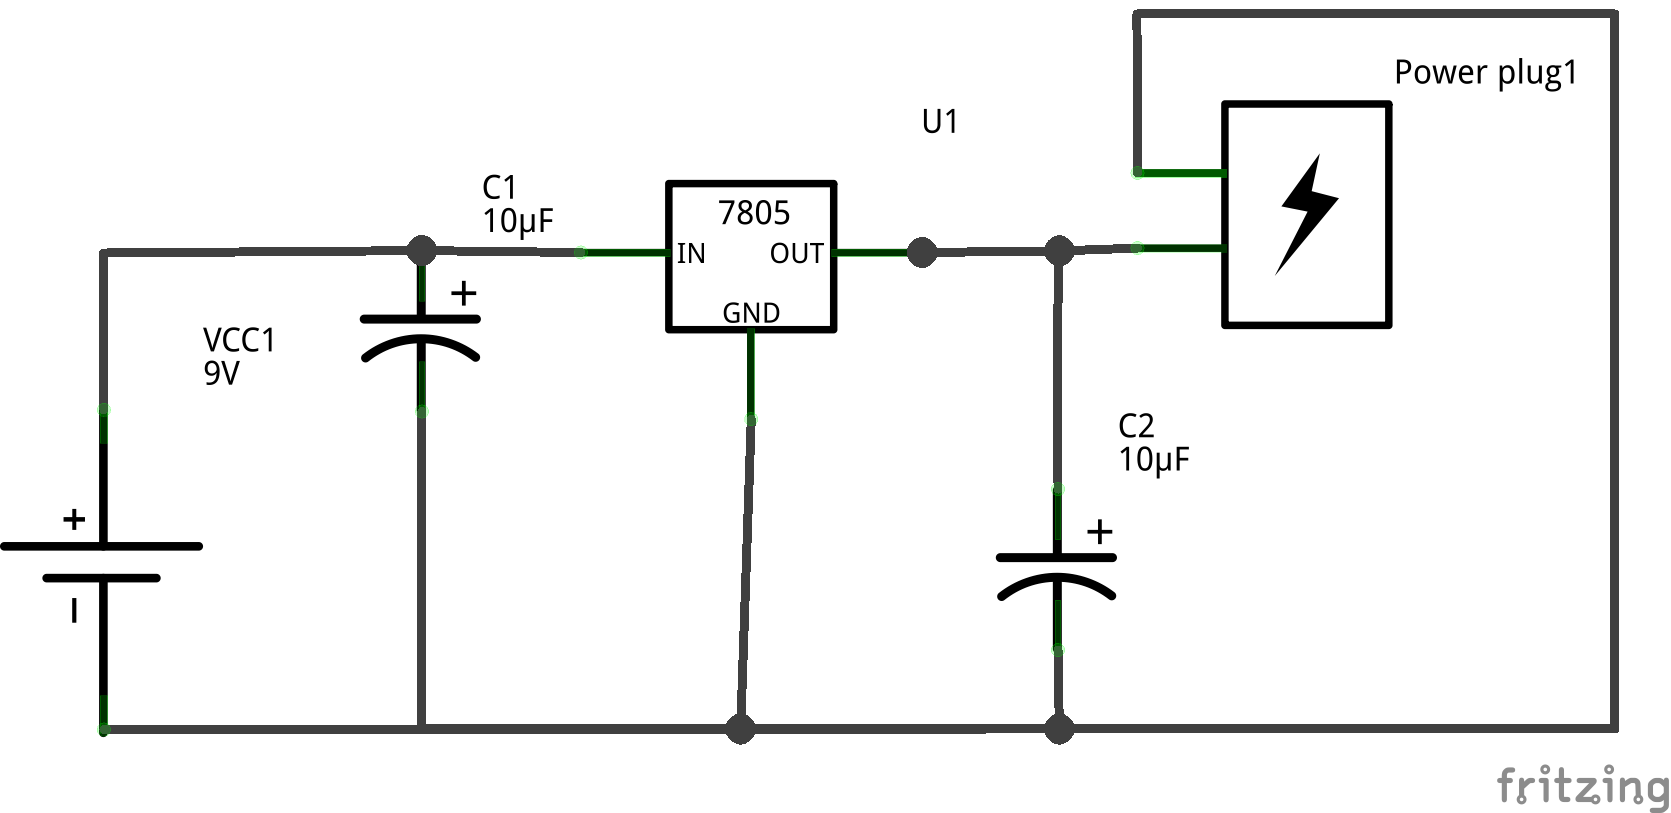
\includegraphics[width=7cm, height=5cm]{fig/esquematrans.png} 
\captionof{figure}{Esquema eléctrico de un transformador de 9V a 5V, utilizando un transistor lm 7805 cv. Los capacitores son electrolíticos de 10 microfaradios.}
\label{fig:g2}
\end{Figure}
\vspace{0.2cm}

\begin{Figure}
\center
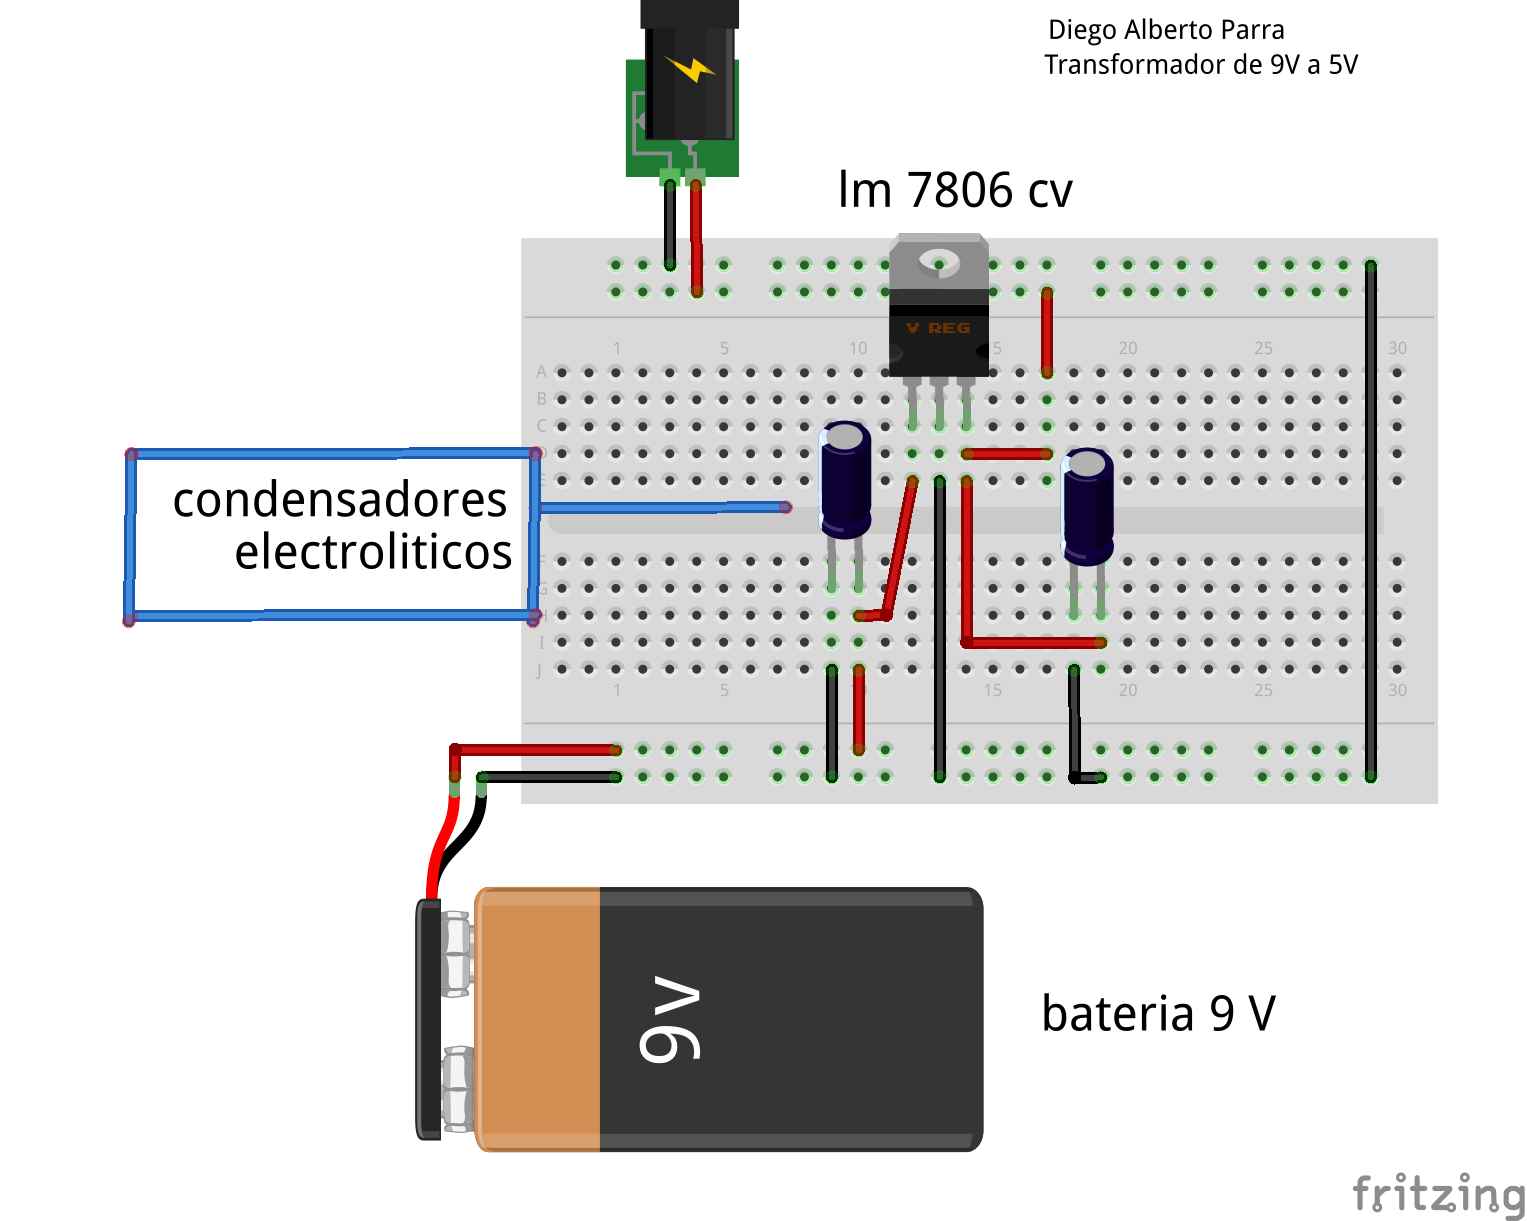
\includegraphics[width=7.cm, height=6cm]{fig/montajetr5V.png}
\captionof{figure}{Montaje en protoboard del circuito regulador de la figura 2.}
\label{fig:g3}
\end{Figure}
\vspace{0.2cm}


El cristal oscilador de 16 mHz debe ir siempre conectado en el microcontrolador, esto  con el fin de ajustar los tres relojes internos que trae el integrado atmega 328 P-Pu, para esto se utiliza el cristal de 16 mHz junto con los dos condensadores cerámicos de 12 picofaradios, Fig. 4 y Fig. 5,  uno de los pines del cristal debe conectarse al pin 9 del microcontrolador y el otro extremo del cristal al pin 10; conectar un capacitor a cada extremo del cristal y los extremos de los capacitores a tierra, de tal forma que los capacitores quedan en paralelo. 
\\ \\
El botón es para reiniciar el microcontrolador en caso de necesitarlo, Fig. 4 y Fig. 5, colocando uno de los extremos del botón, al pin 1 del microcontrolador que es el pin de reset, el otro extremo del botón a una resistencia de 1 Komhs y el extremo de la resistencia a tierra.
\\ \\

\begin{Figure}
\center
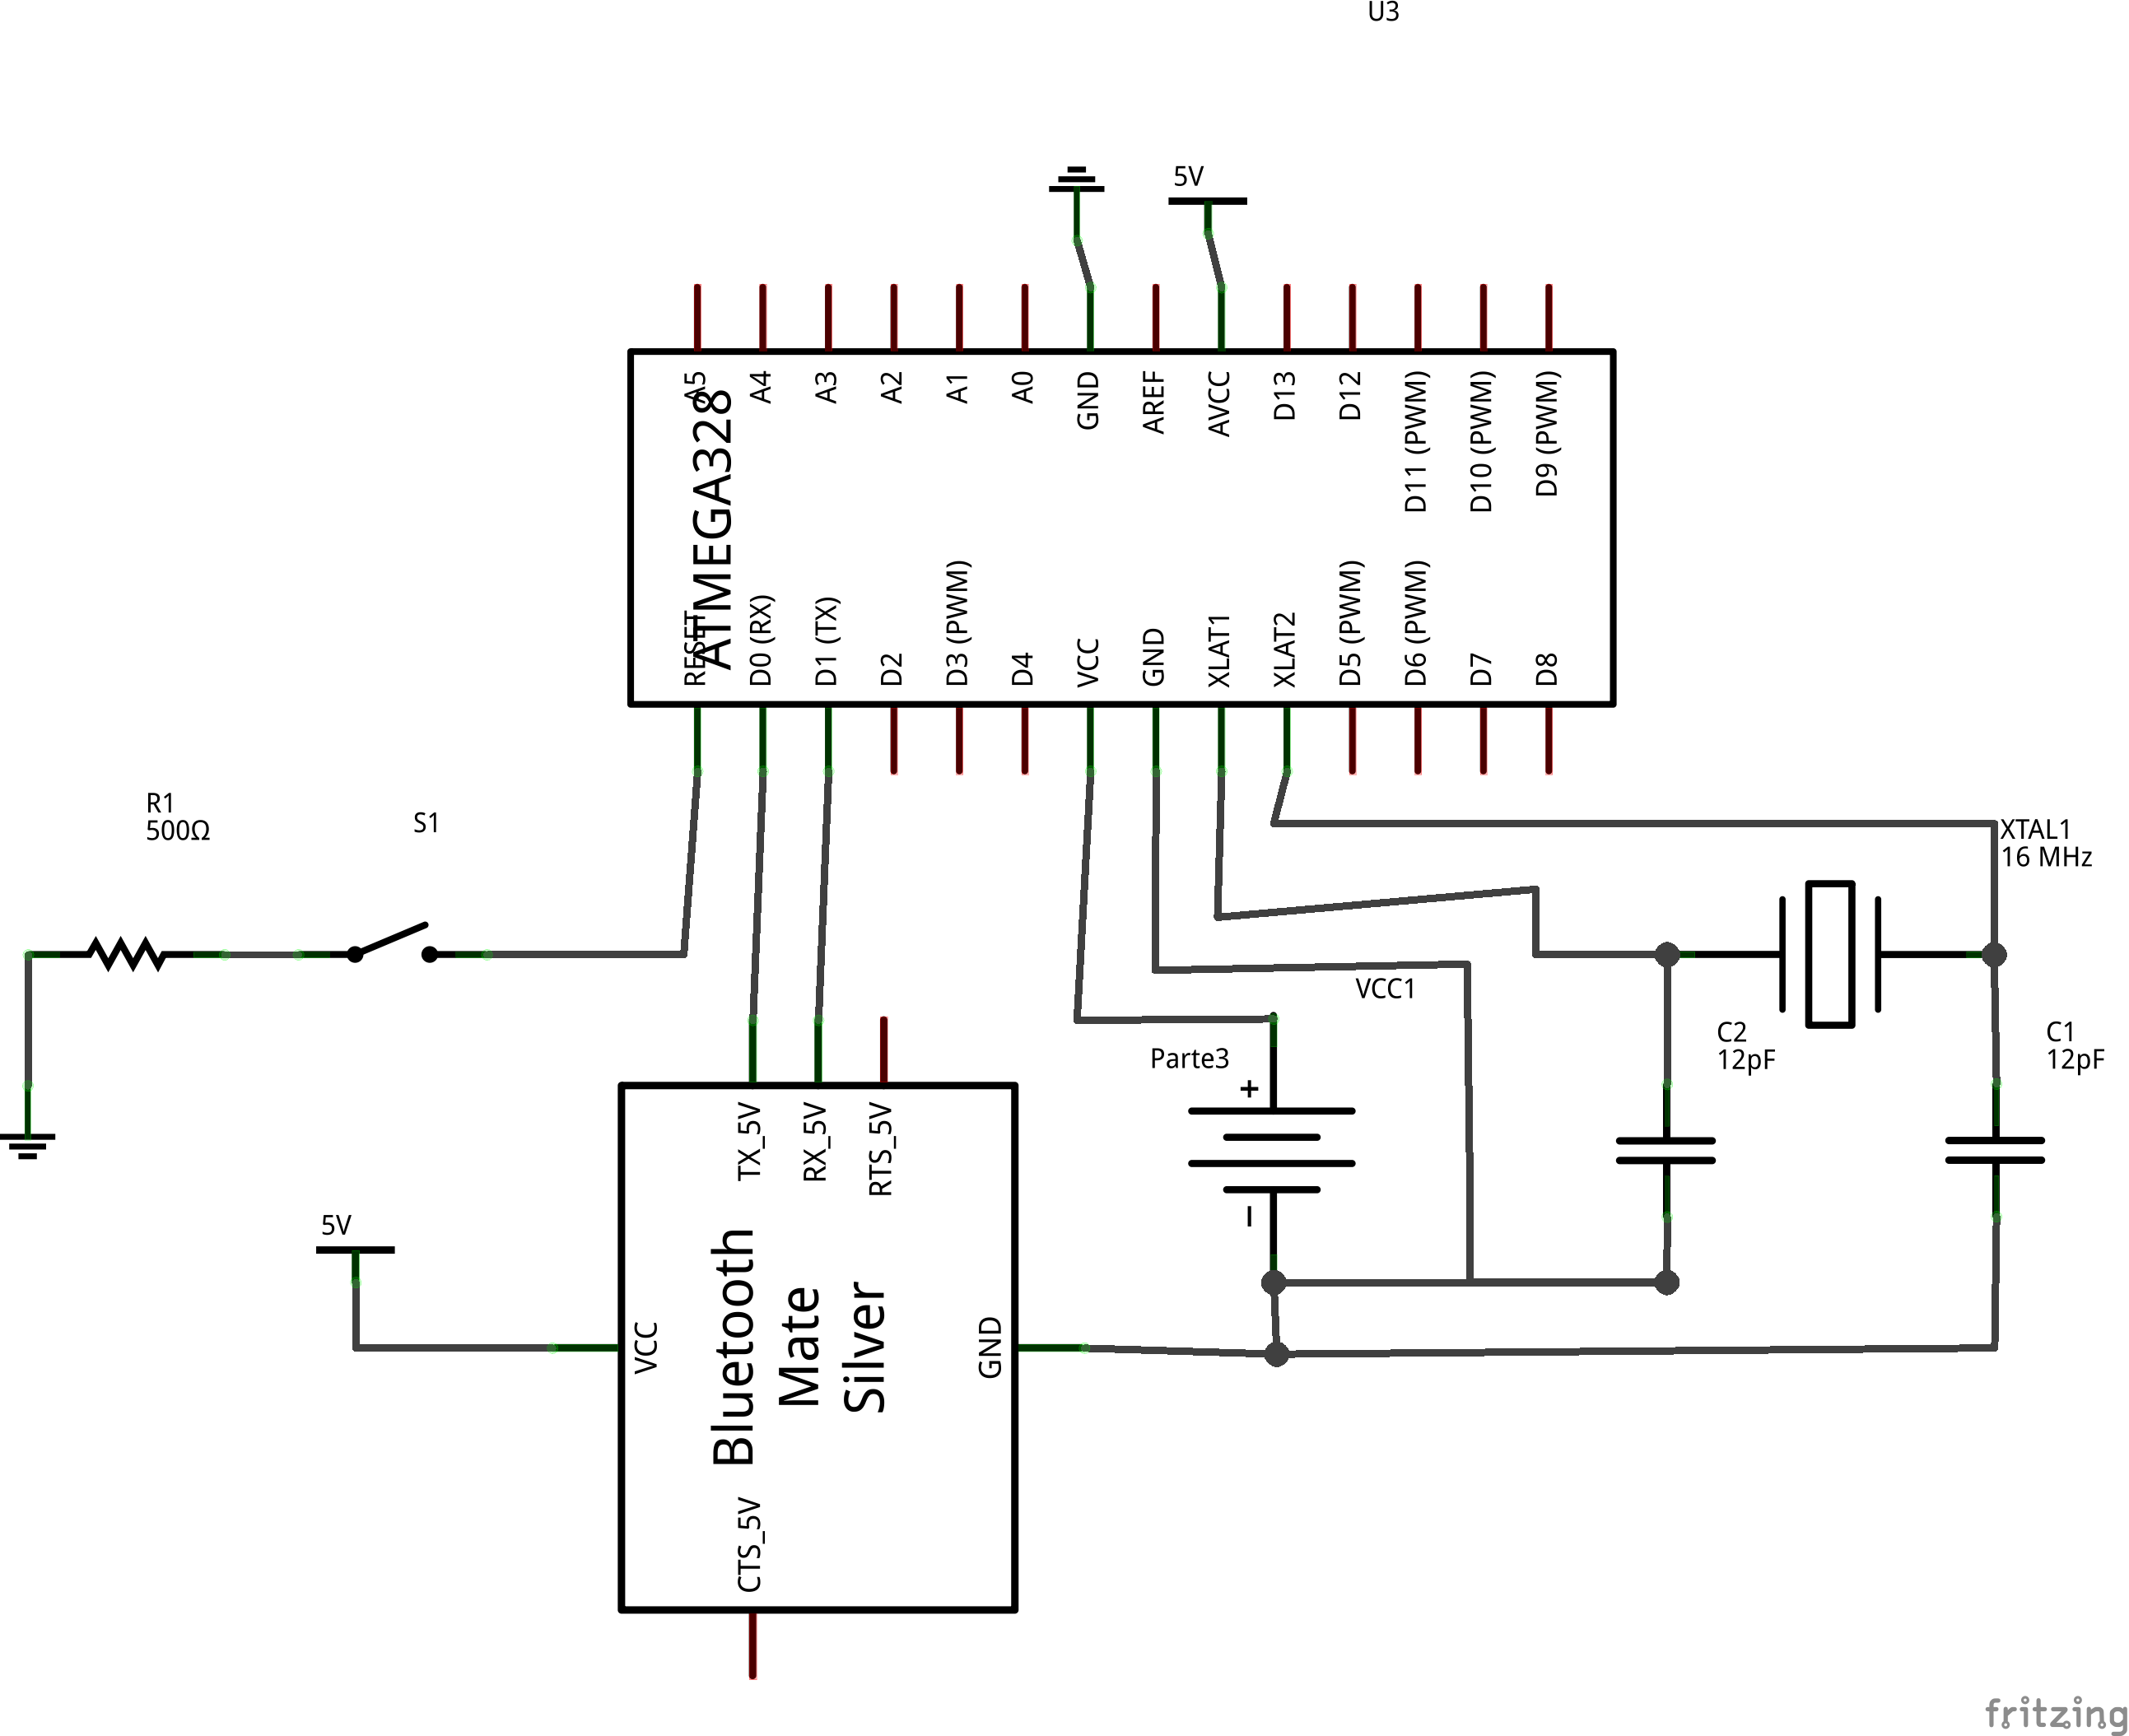
\includegraphics[width=8cm, height=9cm]{fig/bluetoothesq.png} 
\captionof{figure}{Circuito eléctrico modulo bluetooth, conectado a un microcontrolador atmega 328 P-PU junto con un cristal, dos capacitores cerámicos, un botón de reset y una resistencia de 1 Komhs.}
\label{fig:g4}
\end{Figure}
\vspace{1.4 cm}

El modulo bluetooth se debe conectar de la siguiente manera: el pin 2 de la tarjeta arduino es el Rx este va conectado al Tx del blueetooth, el pin 3 del microcontrolador es el Tx y va conectado al pin Rx del bluetooth, Fig. 4 y Fig. 5, el pin GND del bluetooth debe ir a tierra, ahora el pin de Vcc del bluetooth se conecta 5V. 
\\ \\
\begin{Figure}
\center
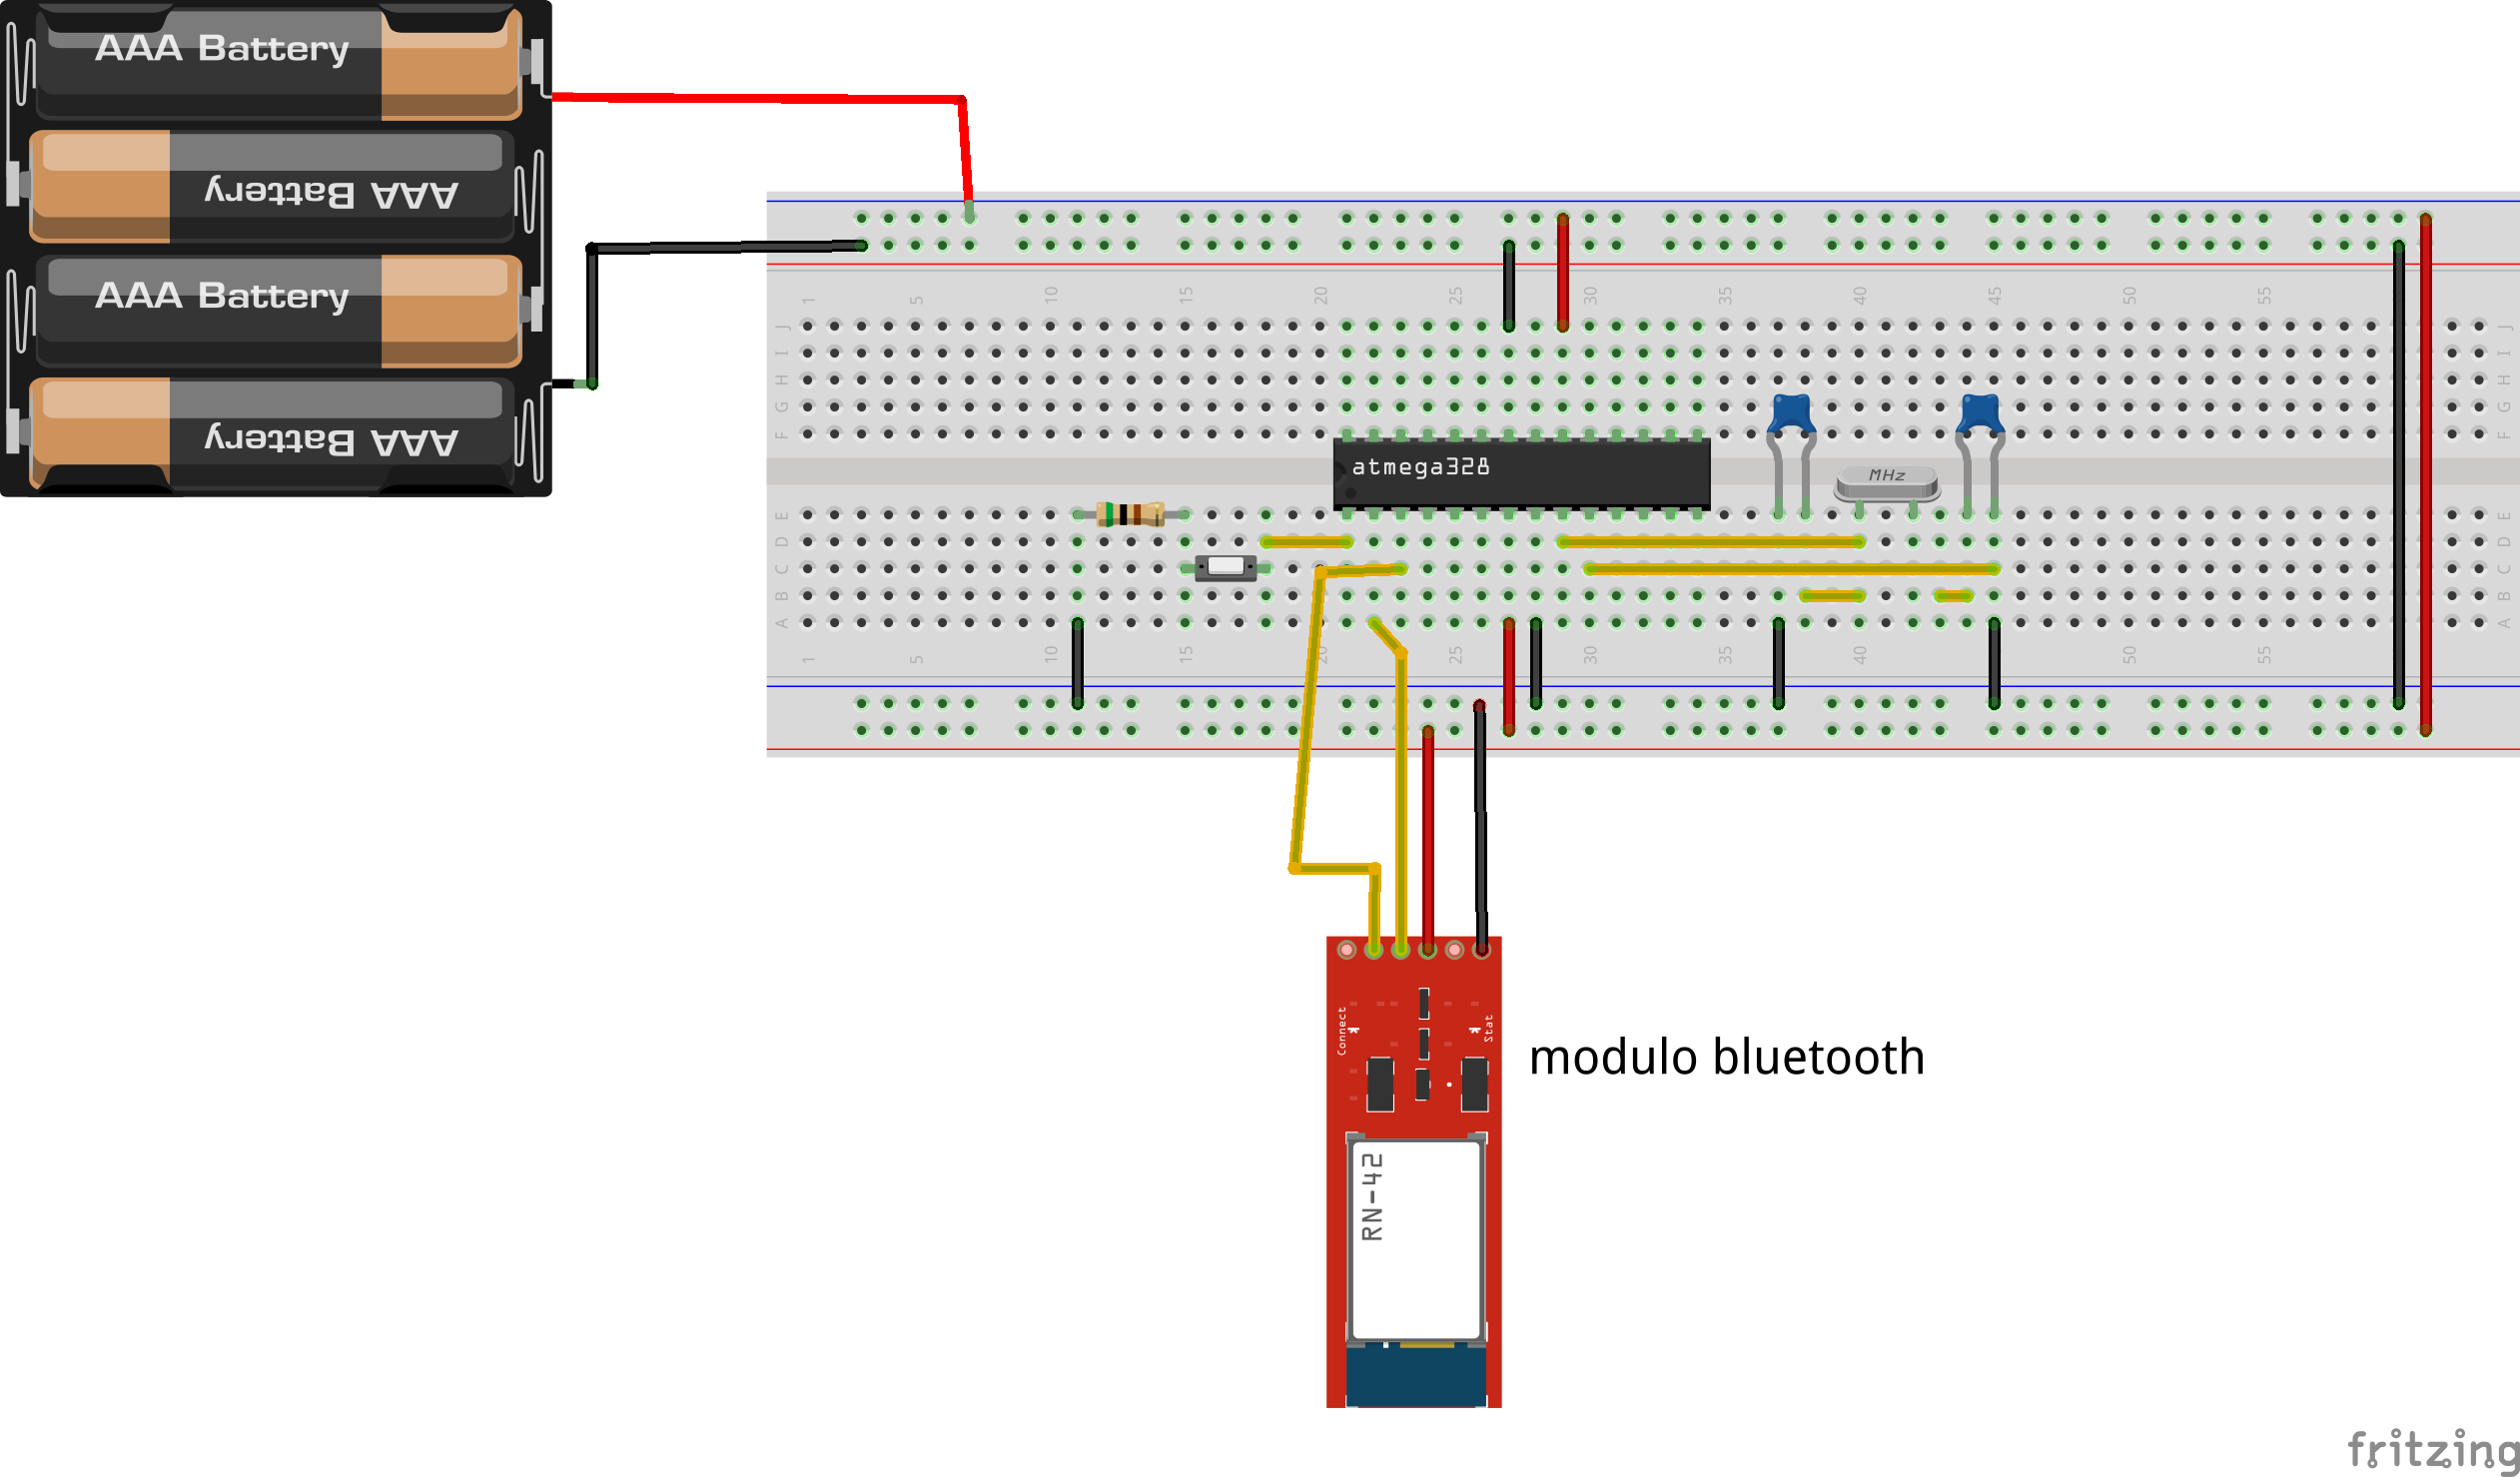
\includegraphics[width=7.cm, height=7cm]{fig/bluetoothmon.png}
\captionof{figure}{Montaje en protoboard del circuito regulador de la figura 4,  los cables negros son tierra, los cables rojos son voltaje, y los cables amarillos son conexiones.}
\label{fig:g5}
\end{Figure}
\vspace{0.2cm}

La parte negativa del diodo  emisor infrarrojo se conecta a un extremo de una resistencia de 500 ohms y el extremo de la resistencia a tierra, figura 6 y 7 ; la parte positiva del diodo emisor se conecta al pin 4 del microcontrolador atmega328, que es la salida digital No. 2. Ahora se conecta la parte positiva del diodo infrarrojo receptor a una resistencia de 1 Komhs y el otro extremo de la resistencia a tierra, se conecta el pin de tierra del diodo receptor infrarrojo a +5V, el pin 28 del microcontrolador conecta a la parte positiva del diodo infrarrojo. 


\begin{Figure}
\center
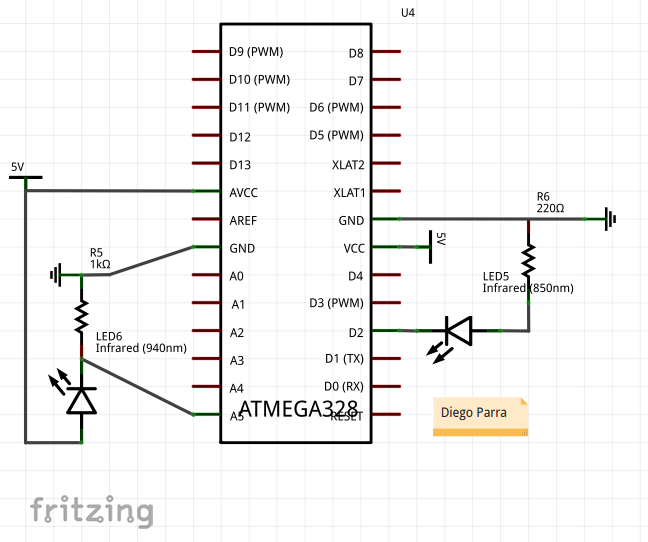
\includegraphics[width=7.cm, height=8cm]{fig/s_esquema.png}
\captionof{figure}{Conexiones de los sensores a la tarjeta micro-controladora atmega328, el diodo receptor infrarrojo es el que se encuentra en la parte izquierda de la figura. El diodo emisor infrarrojo es el que se encuentra en la parte derecha de la figura conectado a tierra a tráves de una resistencia, y, al pin 4 de su otro extremo con el microcontrolador.}
\label{fig:g6}
\end{Figure}
\vspace{0.2cm}



\begin{Figure}
\center
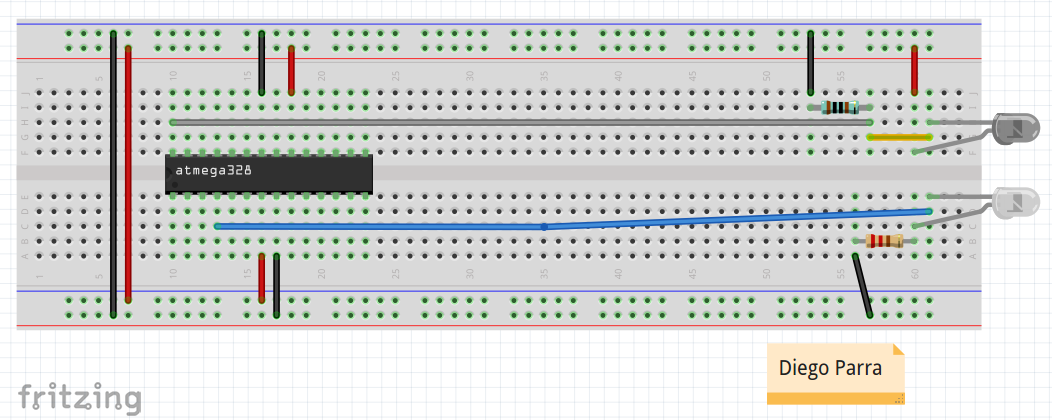
\includegraphics[width=7.cm, height=5cm]{fig/sensores.png}
\captionof{figure}{Montaje en protoboard del circuito los sensores de la figura 6,  los cables negros son tierra, los cables rojos son voltaje, y los cables amarillos son conexiones.}
\label{fig:7}
\end{Figure}
\vspace{2cm}

El led rojo se conecta al pin  9 del microcontrolador, el led verde se conecta al pin 11, el led azul se conecta al pin 10, este montaje con el fin de identificar que proceso se esta realizando en el microcontrolador. Ahora se conectan todos los circuitos anteriormente descritos, en un solo circuito con la baquela para conexiones. figura 8 y 9.  
\\ \\
\begin{Figure}
\center
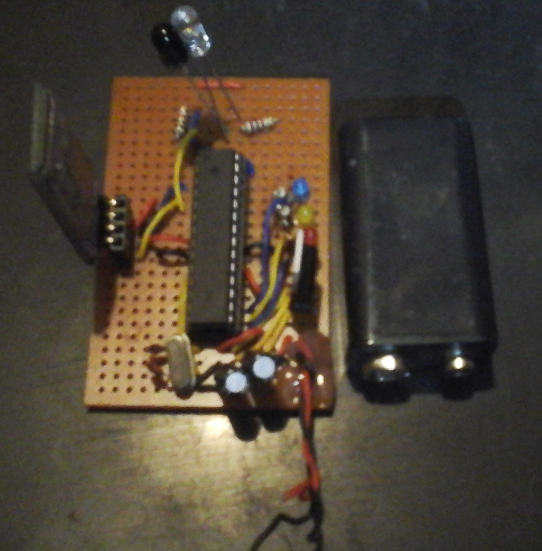
\includegraphics[width=7.cm, height=5cm]{fig/mon0.png}
\captionof{figure}{Montaje en baquela, en la parte superior los diodos tanto emisor como receptor, se colocaron elevados para que la oscilación del péndulo no golpee con ningún componente del montaje.}
\label{fig:8}
\end{Figure}
\vspace{0.2cm}

\begin{Figure}
\center
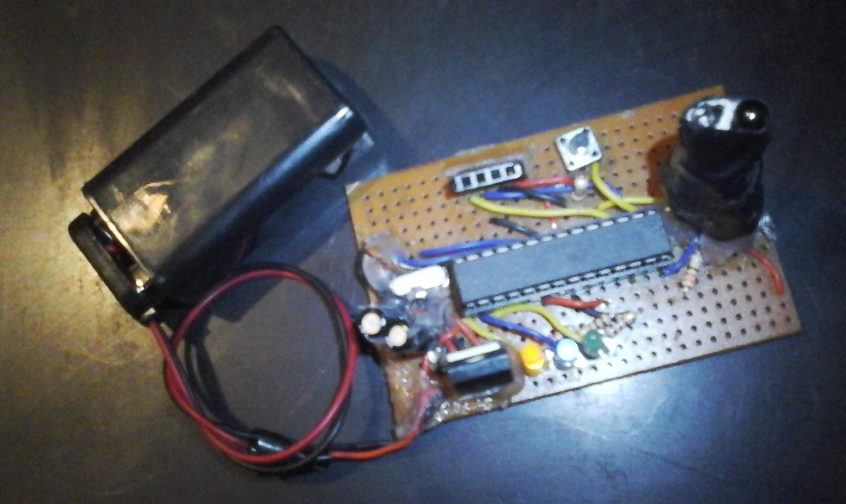
\includegraphics[width=7.cm, height=5cm]{fig/mon1.png}
\captionof{figure}{Montaje final del dispositivo, en la parte derecha superior se coloca un soporte de silicona para los diodos infrarrojos, esto da estabilidad y firmeza, se enrolla con cinta aislante para evitar ruido por radiaciones no deseadas que lleguen transversalmente.}
\label{fig:9}
\end{Figure}
\vspace{0.2cm}

\subsubsection{Instalación del software free pops}
Programa que  ilustra el periodo de oscilación de un péndulo  y calcula la longitud de la cuerda, la frecuencia de oscilación y la frecuencia angular.   Copyright (C) 2015-22-08  Universidad Distrital Francisco Jose, Grupo de física e informática, Dr Julian Andres Salamanca Bernal, Diego Alberto Parra Garzón.
\\ \\ 
El programa free pops es software libre; puedes redistribuirlo y / o modificarlo bajo los términos de la Licencia Pública General GNU publicada por la Fundación para el Software Libre; ya sea la versión 3 de la Licencia, o (a su elección) cualquier versión posterior. 
\\ \\ 
Este programa se distribuye con la esperanza de que sea útil, pero SIN NINGUNA GARANTÍA; ni siquiera la garantía implícita de COMERCIALIZACIÓN o IDONEIDAD PARA UN PROPÓSITO PARTICULAR. Vea el Licencia Pública General GNU para más detalles. 
\\ \\
Para la instalación de free pops es necesario hacer lo siguiente:
\begin{enumerate}
\item[a. ] Abrir una terminal de linux, una vez hecho esto se instala el programa git de la siguiente manera: sudo apt-get install git 
\item[b. ] Descargar el programa free pops de los repositorios de github escribiendo en la terminal: \\git clone https://github.com/Diego-debian/F\\REE\_POPS\_1.0.git 
\item[c. ] Una vez descargado free pops, escribir en la terminal:\\sudo python FREE\_POPS\_1.0/Install/instala\\dor.py 
\item[d. ] Ya abierto el instalador de free pops, pregunta si desea continuar con la instalación escribir 1 y oprimir enter.
\item[e. ] Se despliega un sub-menu que pregunta si desea instalar o desinstalar free pops escribir 1 y oprimir enter.
\item[f. ] El programa actualiza el sistema y pregunta si desea instalar las dependencias de free pops, escribir la tecla S y oprimir enter. 
\end{enumerate}
Una vez hecho esto ya esta instalado el programa. 

\subsubsection{Primer uso de free pops}
Para el primer uso de free pops es necesario:
\begin{enumerate}
\item[a. ] Abrir el gestor de archivos.
\item[b. ] Entrar en la carpeta FREE\_POPS\_1.0.
\item[c. ] Entrar en la carpeta free\_pops.
\item[d. ] Hacer doble click izquierdo sobre el programa free\_pops y escribir la cable de superusuario.
\item[e. ] Conectar la tarjeta arduino uno con el microcontrolador atmega328P-PU, a través del cable usb al computador y oprimir el botón firmware, se abre una ventana de dialogo, oprimir el botón ok. 
\item[f. ] Al abrir la ventana que va a cargar el firmware en el microcontrolador, oprimir el botón continuar, y oprimir el botón ok de la  ventana de dialogo.
\item[g. ] Una vez se inicia la carga del firmware en el microcontrolador aparece una ventana de color azul donde se muestra el estado de la carga del firmware, ver figura 10, al finalizar se cerrara la ventana.
\item[h. ] Oprimir el botón salir.
\item[i. ] Conectar un usb-bluetooth a alguno de los puertos usb del computador y oprimir el botón ON de bluetooth que se encuentra en la parte izquierda del programa, dar ok a la ventana de dialogo.
\end{enumerate}

\begin{Figure}
\center
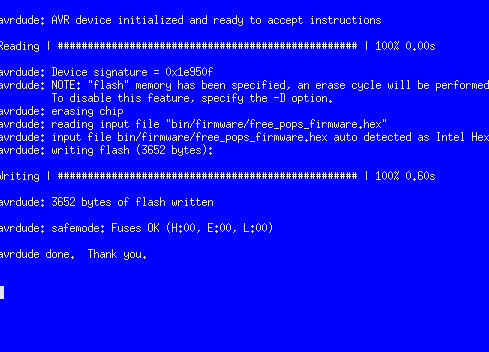
\includegraphics[width=8.cm, height=6cm]{fig/micro.png}
\captionof{figure}{Ventana al terminar de cargar correctamente el firmware en el microcontrolador atmega328P-PU.}
\label{fig:10}
\end{Figure}
\vspace{0.2cm}
  
\subsection{Montaje de laboratorio}
\subsubsection{Materiales}
\begin{enumerate}
\item[a. ] Tres cuerdas de diferentes longitudes cuyo peso sea despreciable.
\item[b. ] Una masa que haga tensión sobre la cuerda.
\item[c. ] Una cinta métrica.
\item[d. ] Montaje eléctrico de free pops.
\item[e. ] Ordenador con Gnu-Linux instalado, conectado a una usb-bluetooth y el software de free pops.
\item[f. ] Un cronometro. 
\item[g. ] Un transportador. 
\end{enumerate}

\subsubsection{Montaje}

\begin{enumerate}
\item[a. ] Uno de los extremos de la cuerda, debe atarse a un eje de giro y el otro a la masa, formando de esta manera un péndulo,  debajo de la masa, debe colocarse el montaje eléctrico de free pops, asegurándose de que los diodos infrarrojos queden a menos de12  centímetros  de la masa.
\item[b. ] El transportador, se  utilizara para medir desde que ángulo se soltara la masa, para comenzar a oscilar.
\end{enumerate}


\end{multicols}
% The bibliography
\begin{thebibliography}{99}
\bibitem{REDISH} Redish, Edward F, \emph{Millikan Award Lecture 1998: Building as cience of teaching physics}, Am. J. Phys. 67 (1999).
\bibitem{GALILEO} Serna, E., José Marquiná, F., \& Fernández, E. GALILEO GALILEI. FACULTAD DE INGENIERÍAS, FUNDACION UNIVERSITARIA LUIS AMIGO.

\end{thebibliography}
\end{document}
